\chapter{Computer Experiments} \label{ch:computer_experiments}

\textbf{A reasonable accurate parameterization should provide a good estimate of the target variable, here cloud cover in isolation. 
Also on a higher level contribute to a improved model performance in the term of uncertainties attributed to a variable or process.}

The results from the experiments conducted based on the setup and configuration presented in Section \ref{sec:hyperparam_tuning}. Finally, each model is evaluated on unseen portion of the dataset presented in the first region.

Unless stated otherwise a model is trained on data in the period 2004 to 2013 and tested on 2014 to 2018. This period was chosen based on the assumption that this is most representable for the climate in the near future.

Although theoretically fascinating it remains to see if \acrshort{lstm} provide a clear practical advantage over the autoregressive models.

Minor differences for the datasets prepared for the \acrshort{ar} and the \acrshort{convlstm}-models. The order of the \acrshort{ar}-model determine the length of the training sequence. All samples with gaps in the requested sequence is disregarded causing a reduction in the data basis for a particular model. For the \acrshort{convlstm} these gaps are filled with a out-of-sample value, $c=1.5$.

\textbf{Make bar plot showing the average number of training and test samples for AR models. This might explain the performans of certain models. }



\section{Framework - Model Setup}
The following sections contain the configurations of the models compiled for this thesis along with descriptions of hyperparameters. A model is compiled based on a choice of hyperparameters. In the search for the best model, different combinations of hyperparameters are tested. This is done manually for \acrshort{ar}-models, and automatically for \acrshort{convlstm}. The \acrshort{ar}-models have a small search space. The \acrshort{convlstm} models have a larger search space and \citepaper{chollet2015kerastuner} provide suitable software. 


\subsection{Autoregressive models}
\textbf{Move first two paragraphs to discussion..?}
The python package ``sciclouds'' provide a self implemented version of \acrshort{ar}-models, using the analytical solution to the least squares problem derived in Section \ref{sec:ARmodels}. 

A set of models are compiled by varying components like scaling the predictors, transforming the target, the inclusion of intercept, order of the models and environmental variables. One AR-model is the combination of 13041 individual regression models. Time consuming task because of the high number of matrix inversions. 

%\subsection{Learning algorithm} \label{sec:backprop_learning_algorithm}
%Learning is a time consuming task. The fundamental trick in deep learning is to use the performance metric as a feedback signal to adjust the weights. It adjusts in the direction of the lowest loss score for the current example (i.e. the current batch). The adjustment is the job of the optimizer, which implements backpropagation algorithmn which is the central learning algoritmn. This section aims to build a understanding of backpropagation trough time without referring to any significant mathematics. If you are interested in the mathematics behind this, read X and Y. 

%\textit{Learning means finding a suitable representation of model parameters that minimize a loss function for a given set of training data samples and their corresponding targets.}

%\section{Notes - Rewrite this entire thing to be "Automatic hyperparameters optimization" }

\subsubsection{Feature Scaling} \label{sec:scaling_predictors}
%Feature standardization makes the values of each feature in the data have zero-mean 

Feature scaling is used to standardise or scale the predictor variables. By subtracting the mean and dividing by the variance, the distribution is reshaped to a standard normal distribution with zero mean and unit variance. Data transformation can be beneficially in an attempt to achieve numerical stability. When applied the predictors is transformed according to the following Equation \ref{eq:scaling_data}. The feature scaling is applied after the partition into training and test dataset, the mean and standard deviation is computed based on the training set. If it was done based on the entire dataset, the trained model would have sneak peaked at the test data.
\begin{equation} \label{eq:scaling_data}
    \mathbf{x} = \frac{\mathbf{x} - \bar{\mathbf{x}}}{\sigma_{\mathbf{x}}}
\end{equation}
where $\bar{\mathbf{x}}$ is the average and $\sigma$ is the standard deviation.
The mean and standard deviation is applied to the test dataset. This is necessary to since the model is now trained to find relations in transformed data, the raw data is out-of-sample.

\subsubsection{Transforming target} \label{sec:transforming_target}
A trick in avioding prediction unphysical values is fitting agains a transformed target. Since the target, \acrfull{cfc}, is within the ranges of 0 and 1. Can be transformed to values from the entire real axis $(-\infty, \infty)$. The inverse transformation truncates the values in the range or [0, 1], alleviation predictions of out-of-sample values. A function suitable for this task is the sigmoid function, shown in figure \ref{fig:activation_func_plus}. 
\begin{figure}
    \centering
    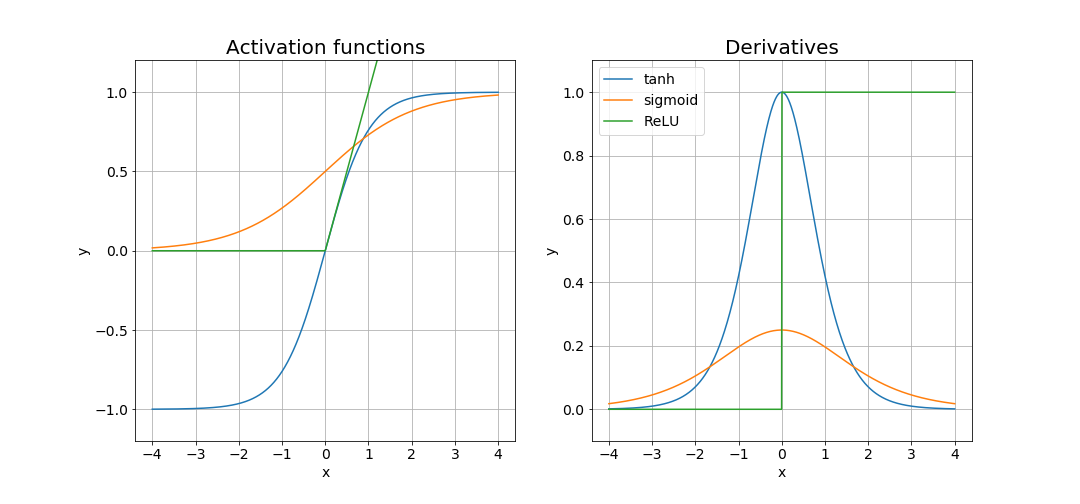
\includegraphics[scale=0.45]{Chapter3_Method/figs/activation_functions_and_derivatives.png}
    \caption{Activation functions used }
    \label{fig:activation_func_plus}
\end{figure}

\subsubsection{Order and Environmental variables}
The dataset for a particular model is a combination of the order, the number of time steps of previous cloud cover includes as predictors and the inclusion of environmental variables, temperature, surface pressure, specific and relative humidity. All model is trained either on the full set of environmental variables or none of them.

\subsubsection{Experimental setup AR-models}
Table \ref{tab:ar_model_config} shows a summary of the \acrshort{ar}-models included in this thesis. 

\begin{table}[h]
    \centering
    \resizebox{\textwidth}{!}{%
    \begin{tabular}{ccccc}
    \cline{2-5}
     & \textbf{Scaling predictors} & \textbf{Transforming target} & \textbf{Order} & \textbf{Enviornmental variables} \\ \hline
    \multicolumn{1}{c}{\textbf{Model 1}} & \checked & $\times$  & 1 & $\times$ \\ \hline
    \multicolumn{1}{c}{\textbf{Model 2}} & \checked & $\times$  & 0 & \checked   \\ \hline
    \multicolumn{1}{c}{\textbf{Model 3}} & \checked & $\times$  & 1 & \checked  \\ \hline
    \multicolumn{1}{c}{\textbf{Model 4}} & \checked & $\times$  & 2 & \checked  \\ \hline
    \multicolumn{1}{c}{\textbf{Model 5}} & \checked & $\times$  & 3 & \checked  \\ \hline
    \multicolumn{1}{c}{\textbf{Model 6}} & \checked & $\times$  & 4 & \checked  \\ \hline
    \end{tabular}%
    }
    \caption{Configuration of \acrshort{ar}-models. $\times$ denoted not applied, \checked denotes applied}
    \label{tab:ar_model_config}
\end{table}


\subsubsection{Varying the test sample}
% Prøv å gjøre dette plottet ikke en hel side da er det lettere for latex å plassere det tror jeg.
Partition into test-datset, remaining data is used for training. 
\begin{itemize}[noitemsep, topsep=0pt]
    \item Test 1 : 2014 - 2018
    \item Test 2 : 2009 - 2013
    \item Test 3 : 2004 - 2008
\end{itemize}

\subsection{Convolutional LSTM}
% Endrer på arkitekturen - denne bruker -train - validation - test, en hvis prosentandel a
The formulation of the Air quality forecasting problem presented by  \citeauthor{SunAirLSTM} is similar to the formulation of the cloud fractional cover prediction problem presented in this project. The machine learning experimental setup is adopted from the paper \citepaper{SunAirLSTM}. The model names is given following this structure, described using a example. The model \textit{ConvLSTM 3x3-256-2}, is a \acrshort{convlstm} model using a $3\times 3$ filter, 256 hidden states and has 2 layers. A hyper parameter is a constant set before the training procedure begins. There is a mind-boggling amount of choices for hyperparameters, the initial configuration used in the conducted experiments for this project draw inspiration from this paper. 

\subsubsection{Automatic hyperparameter optimisation}  \label{sec:hyperparam_tuning}
The more complicated models would further benefit from a automatised tuning routine, making desitions based on certain criterias.
%\textit{Learning to forget found the best accuracy when using learning rate decay.}
The keras tuner used in this thesis, make decisions based on X. Batch size describes the number of samples used to make a weight update. The number of epochs determines how many times the datasets sees all samples. The learning rate determines the magnitude of the step taken in the direction of the steepest gradient, as described in Section X. The optimiser is the algoritmn desiding the weight update. \textbf{Kept constant and describe this}. All models use the MSE loss in combination with the Adam optimiser. The list describes models tested in this experiment. 

\begin{enumerate}[noitemsep, topsep=0pt]
    \item ConvLSTM 1x1-256-2
    \item ConvLSTM 3x3-256-2
    \item ConvLSTM 5x5-256-2
    \item ConvLSTM 3x3-256-3
    \item ConvLSTM 5x5-256-3
\end{enumerate}

\textbf{Trenger du hyperparameteroptimisering når du bruker den artikkelen?}

\section{Results}

\subsection{Autoregressive models}

%%%% TARGET PREDICITON HORIZONTAL
\begin{figure}[ht]
    \centering
    \includegraphics{python_figs/target_prediction_plot_horizonal.pdf}
    \caption{Comparison target and predicted cloud fractional cover.}
    \label{fig:target_predict_horizontal}
\end{figure}

%%%% TARGET PREDICITON HORIZONTAL
\begin{figure}[ht]
    \centering
    \includegraphics{python_figs/target_prediction_plot_vertical.pdf}
    \caption{Comparison target and predicted vertical cloud fractional cover.}
    \label{fig:target_predict_vertical}
\end{figure}

%%%% TARGET PREDICITON ERA5
\begin{figure}[ht]
    \centering
    \includegraphics{python_figs/target_prediction_era5_plot_horizonal.pdf}
    \caption{Comparison target, predicted and era5 horizontal cloud fractional cover.}
    \label{fig:target_predict_era5_vertical}
\end{figure}

\subsection{\acrlong{convlstm} }
Either summaries the findings into one table 

%\chapter{Discussion}

\subsection{Testing?}

\section{Experiments}



The statistical properties are slightly different for the different test sets.  

Short sequnece length to reduce the computational com-
plexity of experiments. 

No efforts have been made to assess the impact of the artefact on the performace.

One variable was not found to increase the performance.


data sets can be reduced without significant loss of information

A drawback of this study was not to account for correlations between radiomics features and the ROI, but such corrections were
not performed in this thesis.

Land ocean mask study statistics of subgroups.


\section{Practical implications - OUTDATED} \label{sec:practical_implications}
It is necessary to have a understanding of the needs of the end product before conducting large machine learning projects. Answering questions like: What will it be used for and how can it be implemented in useful way?

A major downside of the data driven learning approach is the rigid resolution. A trained model can only be used on similar problems, with the same spatiotemporal resolution. For applications like climate models, output comes in a wide range of different resolutions. Before implementing the finished product in a new model of a different resolution, it would need to be retrained on the resolution of the climate model under development. This process involves both remapping of the dataset and retraining the model at the correct resolution. This is a time consuming process involving finding a new set of hyperparameters suitable for the new resolution. % It essentially means starting over.

Once trained on global climate datasets, machine learning models provide fast results even for complex parameterization which is what makes them suitable for the application of climate modelling. Most machine learning packages are developed using Python. \acrfull{esm} are implemented in python. Methods for including the trained parameterizations need to be developed.
 
\subsection{Any implications based on the results presented in this chapter.}